\documentclass[12pt,oneside,spanish]{article}
\usepackage[T1]{fontenc}
\usepackage{times}
\usepackage[utf8]{inputenc}
\usepackage[a4paper]{geometry}
\geometry{verbose,tmargin=2cm,bmargin=2cm,lmargin=3.5cm,rmargin=2cm}
\setcounter{secnumdepth}{3}
\setcounter{tocdepth}{3}
\usepackage{color}
\usepackage[spanish,es-tabla]{babel} % Tabla instead of Cuadro in spanish
\usepackage{amssymb}
\usepackage{amsmath}
\usepackage{psfrag}
\usepackage{multirow}
\usepackage{graphicx}
\usepackage{subfigure}
\usepackage{longtable}
\usepackage{dcolumn}
\usepackage{booktabs}
\usepackage{listings}
\usepackage[unicode=true,linkbordercolor={1 1 1}]{hyperref}
% References styles fo bibtex

\lstdefinestyle{python}{
    texcl=true,
    language     = python,
    tabsize=4,
    escapeinside=@@,
    basicstyle   = \scriptsize\ttfamily,
    keywordstyle = \bfseries,
    keywordstyle = [2]
    commentstyle = \color{MEtitle},
   morekeywords=[1]{
      library, use ,all,entity,is,port,in,out,end,architecture,of, body,
      function, variable, begin,and,or,Not,downto,ALL, signal, process, if,
      else, elsif, case, when, then, range, to, component, type, with, select,
      others, constant, inout, buffer, map, true, false, array, subtype, wait,
      wait for, generic, =, <, >, <=, >=, =>,
   },
   alsoletter={=, <, >},
   morekeywords=[2]{
          STD_LOGIC_VECTOR,STD_LOGIC,IEEE,STD_LOGIC_1164, work, local, real,
          math_real, time, NUMERIC_STD,STD_LOGIC_ARITH,STD_LOGIC_UNSIGNED,
          std_logic_vector, std_logic, ieee, numeric_std, std_ulogic,
          std_logic_1164, natural, bit, bit_vector, signed, unsigned,
          boolean, integer
    },
    morekeywords=[3]{rising_edge, falling_edge, resize, to_signed, to_unsigned},
    morecomment=[l]{--},
}

\bibliographystyle{abbrvnat}

% Chapter
\usepackage{titlesec}
%\titleformat{\chapter}[block]{\bfseries\scshape\Huge}{}{0pt}{\filcenter}[]
\titleformat{\chapter}[block]{\bfseries\Huge}{}{0pt}{\filcenter}[]

% Heading
\usepackage{fancyhdr}
\pagestyle{fancy}
%\renewcommand{\chaptermark}[1]{\markboth{#1}{}}
%\renewcommand{\sectionmark}[1]{\markright{--- #1}}
\fancyhf{}   %apaga tudo
\fancyhead[C]{\scriptsize\scshape\nouppercase{\leftmark}}
\fancyhead[R]{\oldstylenums\thepage}
\renewcommand\headrulewidth{0pt}
\fancypagestyle{plain}{
	\fancyhead[R]{\bfseries{\oldstylenums\thepage}}
	\fancyhead[C]{}}

% Turn table
\usepackage{fancybox}

% Title page
\title{ 
	
\includegraphics[width=0.35\textwidth]{unsa.eps}\\
	\vspace{0.1cm}
{\large Escuela Profesional de Ingeniería Electrónica \\
\vspace{2cm}
{\small Guía de Laboratorio de Tecnología de la Ingeniería Aeronáutica y Espacial}} \\ 
\vspace{0.1pt} 
\hrulefill \vspace{40pt} \\ 
\textbf{Lab 01: Cinemática de los Sistemas Aeroespaciales}\\ 
\vspace{30pt} \hrulefill}
\author{\scshape{\textbf{ }}
\vspace{30pt} \\
	\vspace{0.5cm}
	{\small Alumnos}\\
	{\Large Dolmos Becerra, Uriel Frankdali}\\
	{\Large Pocohuanca Fernandez, Jeremin}\\
	{\Large Torres Cori, Josue Breithner}\\
	\vspace{3cm}\\
{\small Profesor: Dr. Juan C. Cutipa Luque}\\
\vspace{20pt}
}
\date{6 de mayo de 2021}

\begin{document}

\pagenumbering{gobble}

\maketitle

\newpage



\pagebreak

\tableofcontents
%\listoffigures
%\listoftables

\newpage
\pagenumbering{arabic}

%  ---------------------- here goes your report -------------
%
\section{Objetivo}
Entender los diferentes sistemas de coordenadas usados en el estudio de la cinemática de los sistemas aeroespaciales.
\section{Fundamento Teórico}
En esta parte, el alumno recolecta la información necesaria para realización de su experiencia. La fuente principal de información es el contenido de la unidad 1 según sílabo de la asignatura de Tecnología de la Ingeniería Aeronáutica y Espacial.

\section{Materiales y Equipamientos}
\begin{itemize}
    \item Computador Laptop.
    \item Gnu-Octave\footnote{Software libre que se distribuye bajo la licencia GPL ver 3, disponible en \url{https://www.gnu.org/software/octave/}}.
    \item Python 2 y Python 3\footnote{Este lenguaje de programación es uso libre y está disponible en \url{www.python.org}}.
    \item Cocalc, plataforma basada en web para desarrollo de algoritmos en la nube (disponible en \url{https://cocalc.com}).
\end{itemize}

\section{Procedimientos}
Los procedimientos de la presente experiencia de Laboratorio son:
\begin{enumerate}
\item Crear una cuenta en Cocalc, usando el correo institucional.
\item Crear un proyecto de nombre 'Lab 01 TIAE 2021 A' (ver Fig. \ref{fig:crearProyecto}). Ingrese al proyecto creado y cree un nuevo archivo de nombre 'lab01primer.py' (ver Fig. \ref{fig:crearPrograma})

\begin{figure}[h]
    \centering
    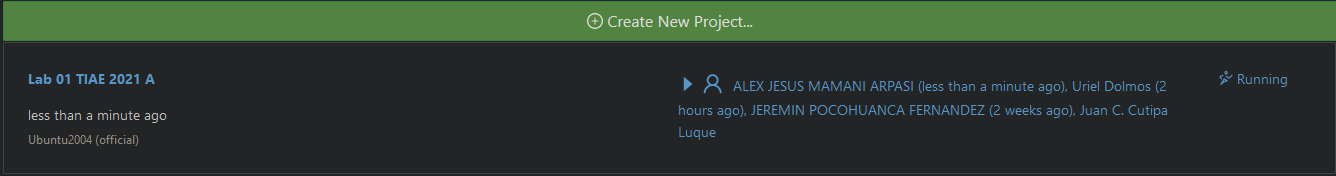
\includegraphics[scale=0.4]{Codigo/2.Proyecto.png}
    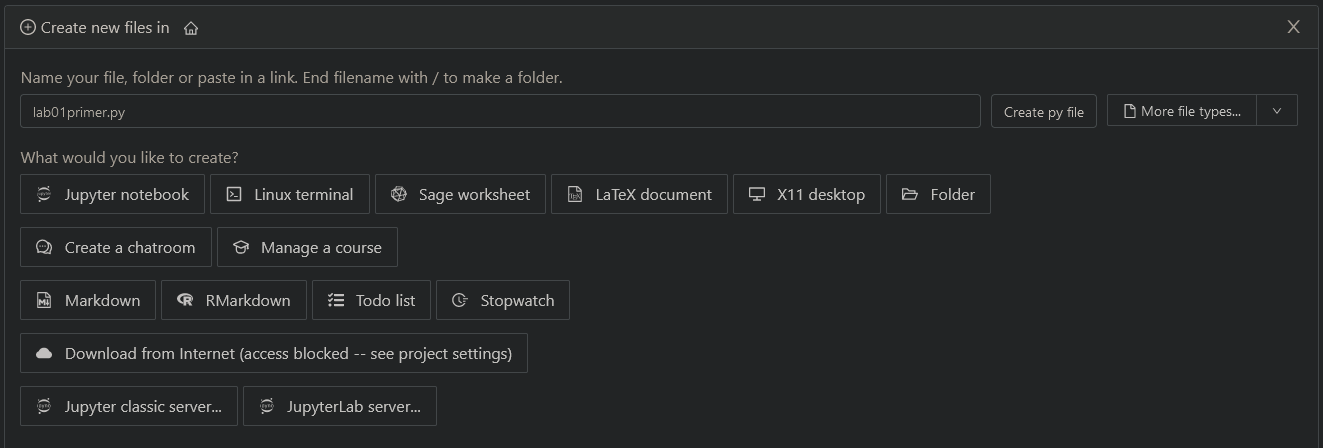
\includegraphics[scale=0.4]{Codigo/2.archivo.png}
    \caption{Creación del proyecto}
\end{figure}

\item Clicar sobre el nombre del archivo creado y en la ventana de código que aparecerá, realice su primer programa. Use el icono de la derecha 'Split frame vertically ...' para configurar la ventana de "terminal", o el equivalente a CMD de Windows.

\begin{figure}[h]
    \centering
    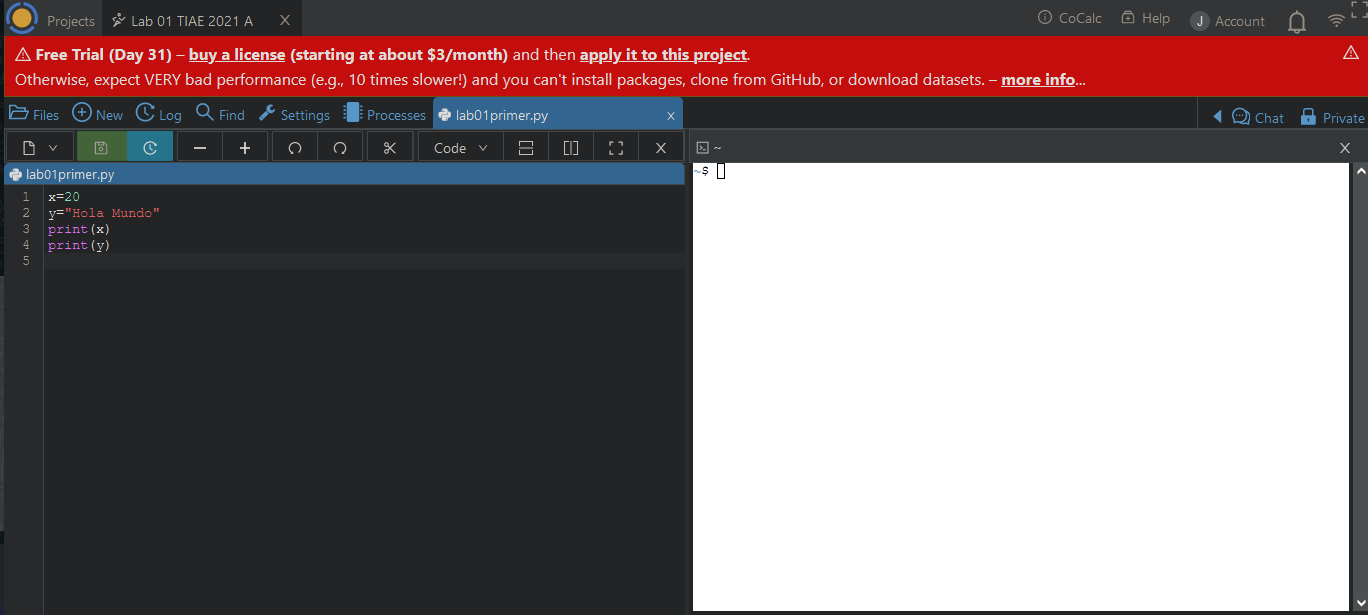
\includegraphics[scale=0.4]{Codigo/3.terminal.png}
    \caption{Abrir Terminal}
\end{figure}

\item Ejecute el programa 'lab01primer.py', desde la ventana de 'terminal' digitando '~\$ python lab01primer.py' (Ver Fig. \ref{fig:primer}). En posteriores programas, deberá sustituir 'python' por 'python3', ya que es la versión más actualizada.

\begin{figure}[h]
    \centering
    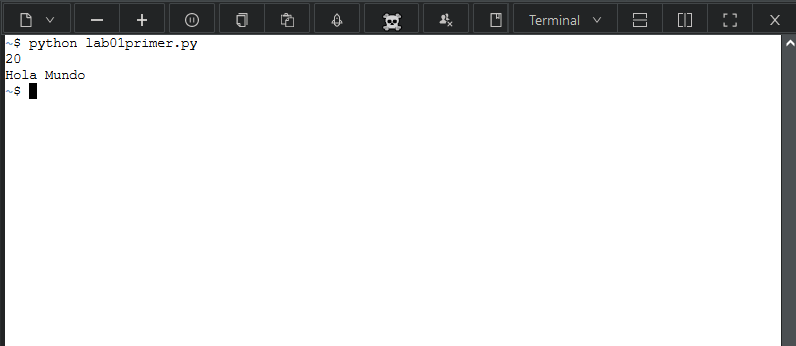
\includegraphics[scale=0.7]{Codigo/4.Ejecutar.png}
    \caption{Ejecutar programa}
\end{figure}

\item Realizar un programa para calcular la matriz de rotación siguiente \cite{fossen:2011}:

$R{x} = \begin{pmatrix} 1 & 0 & 0 \\ 0 & \cos\phi & -\sin\phi \\ 0 & \sin\phi & \cos\phi \end{pmatrix}$
\\
\begin{lstlisting}[language=Python,numbers=left,numbersep=5pt,numberstyle=\tiny, frame=single]
import numpy as np
import math as m
  
def Rx(phi):
  return np.matrix([[ 1, 0        , 0          ],
                    [ 0, m.cos(phi),-m.sin(phi)],
                    [ 0, m.sin(phi), m.cos(phi)]])

phi = m.pi/2

print("the test angle, phi =", phi)
  
R = Rx(phi)
print(np.round(R, decimals=2))
\end{lstlisting}

\lstinputlisting[style=python, frame=single]{Codigo/RotacionMatrizRx.py}

\item Realizar un programa para calcular la matriz de rotación siguiente \cite{fossen:2011}:

$R{y} = \begin{pmatrix} \cos\theta & 0 & \sin\theta \\ 0 & 1 & 0 \\ -\sin\theta & 0 & \cos\theta \end{pmatrix}$

\lstinputlisting[style=python, frame=single]{Codigo/RotacionMatrizRy.py}

\item Realizar un programa para calcular la matriz de rotación siguiente \cite{fossen:2011}:

$R{z} = \begin{pmatrix} \cos\psi & -\sin\psi & 0 \\ \sin\psi & \cos\psi & 0 \\ 0 & 0 & 1 \end{pmatrix}$

\lstinputlisting[style=python, frame=single]{Codigo/RotacionMatrizRz.py}

\item Implementar un programa que calcule la matriz $\mathbf{J_\theta (\eta)}$ de transformación presente en la ecuación (2.40) de \cite{fossen:2011}. 

\lstinputlisting[style=python, frame=single]{Codigo/MatrizJ.py}

\item Realizar un programa que realice la transformación de coordenadas de NED a Body.
\item Realizar un programa que realice la transformación de coordenadas de ECEF a Body.
\item Realizar un programa que realice la transformación de coordenadas de ECEF a NED.
\end{enumerate}

\textbf{Recomendación:} Debe incluir al profesor (jccluque@gmail.com) como colaborador de su proyecto en Cocalc.
\section{Cuestionario}
Se anexan los datos de un experimento de un vehículo acuático de superficie no tripulado. Usar los programas anteriores y obtener los datos en coordenadas:
\begin{enumerate}
    \item BODY frame.
    \item ECEF frame.
    \item NED frame.
\end{enumerate}
\textbf{Obs.} Cuando no hay interrogantes, se recomienda discutir los resultados obtenidos durante el procedimiento de la experiencia.

\begin{figure}
    \centering
    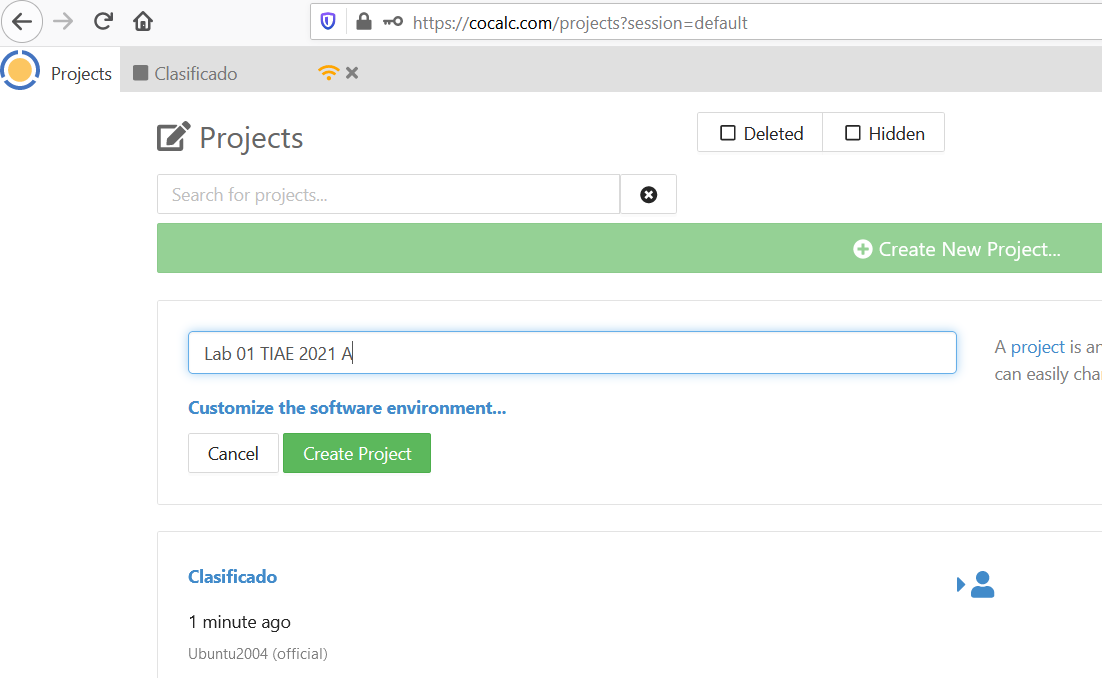
\includegraphics[width=12cm]{crearProyecto.png}
    \caption{Crear Proyecto en Cocalc.}
    \label{fig:crearProyecto}
\end{figure}

\begin{figure}
    \centering
    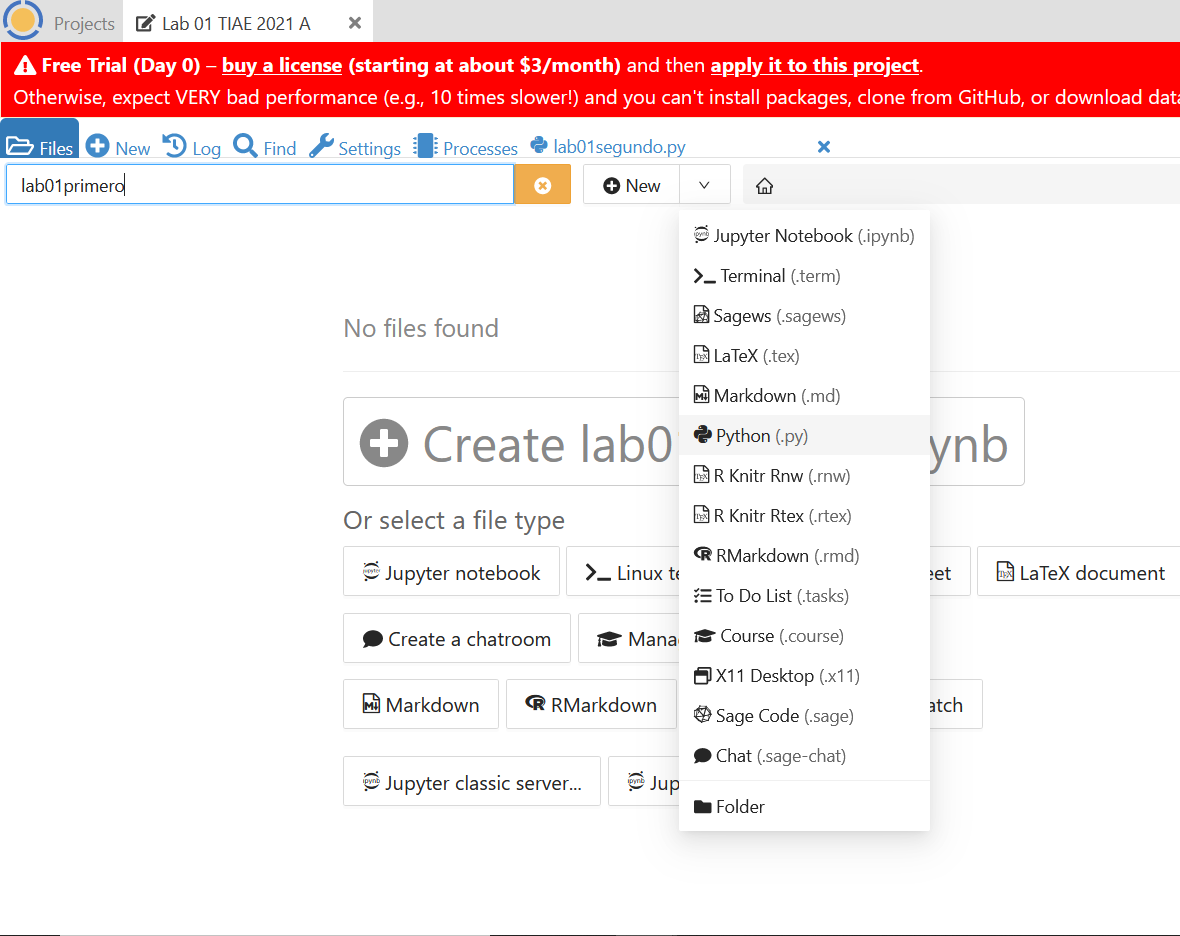
\includegraphics[width=12cm]{crearPrograma.png}
    \caption{Crear Programa dentro de Proyecto en Cocalc.}
    \label{fig:crearPrograma}
\end{figure}

\begin{figure}
    \centering
    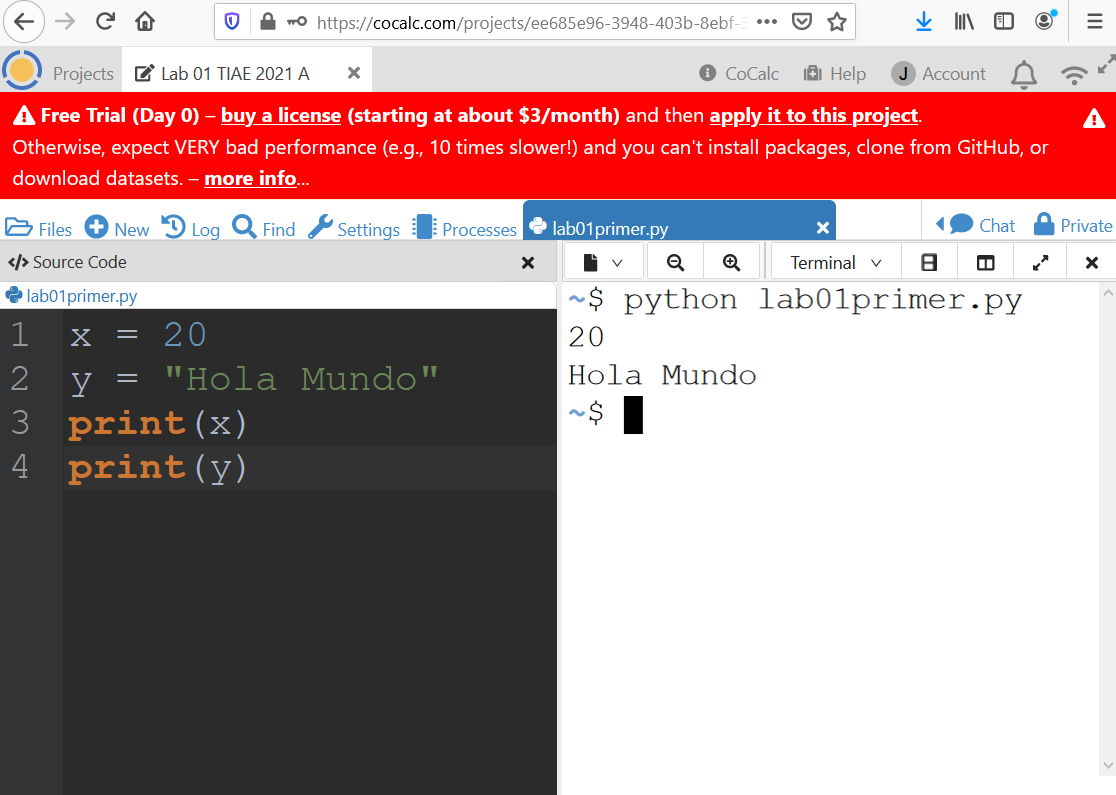
\includegraphics[width=12cm]{primer.png}
    \caption{Primer programa en python.}
    \label{fig:primer}
\end{figure}



\section{Conclusiones}
Aquí debe concluir de forma sucinta sobre la experiencia realizada y colocar observaciones que considere pertinentes.
Puede encontrar más información en las referencias del silabo del curso o en el texto de \cite{fossen:2011}.

\begin{itemize}

    \item Se ejecutaron en la nube los programas que escribimos en lenguaje python gracias a la plataforma Cocalc
    \item 
    
\end{itemize}

\section{Repositorio}
\begin{itemize}
    \item Github: 
    \url{https://github.com/jtorrescor/Lab-01-TIAE-2021-A}.
    \item Latex: 
    \url{https://es.overleaf.com/project/60a71a3436b8449fd57e5ff0}.
\end{itemize}

\newpage
%\fancyhead[C]{\scriptsize\scshape\nouppercase{\leftmark}}
\addcontentsline{toc}{section}{Referencias Bibliográficas} %
%

\bibliography{referencias}
\appendix


\newpage
\addcontentsline{toc}{section}{Apéndice} %
\section*{Apéndice}

\newpage
\addcontentsline{toc}{section}{Rúbrica} %
\section*{Rúbrica}
\begin{itemize}
\item[e1:] Identifica y diagnostica problemas y los prioriza de acuerdo a su impacto o relevancia.
\item[e2:] Formula soluciones coherentes y realizables usando normas y estándares apropiados.
\item[e3:] Utiliza las técnicas y metodologías de la ingeniería electrónica para plantear, analizar y resolver problemas de ingeniería.
\item[e4:] Maneja equipos e instrumentos y utiliza software especializado propio del ejercicio profesional.
\end{itemize}
La tabla \ref{tab:rubricas} refleja la evaluación del estudiante respecto este informe y mediante entrevistas. 

\begin{table}[h!]
\caption{Rúbrica según Resultados del Estudiante}
\centering
\begin{tabular}{lcccc}
\hline 
Alumno & e1 & e2 & e3 & e4\tabularnewline
\hline 
\hline 
Dolmos Becerra, Uriel Frankdali &  &  &  & \tabularnewline
\hline 
Pocohuanca Fernandez, Jeremin &  &  &  & \tabularnewline
\hline 
Torres Cori, Josue Breithner &  &  &  & \tabularnewline
\hline
\end{tabular}
\label{tab:rubricas}
\end{table}
\end{document}


